\documentclass[12pt]{article}

\newcommand\floor[1]{\lfloor#1\rfloor}
\newcommand\ceil[1]{\lceil#1\rceil}

\usepackage{amsmath}
\usepackage[super]{nth}
\usepackage[utf8]{inputenc}
\usepackage[T1]{fontenc}
\usepackage{textcomp}
\usepackage{gensymb}
\usepackage{graphicx}

\pagenumbering{arabic}

\begin{document}

\title{Music Generation in ArtToMusic}
\date{February 22, 2017}
\author{Rafael De Smet}

\maketitle
\tableofcontents

\section{Introduction}

In this paper I will discuss several methods to generate music with software. Analogous to the paper in graphical analysis, I will discuss methods I use in the ArtToMusic project and methods I did not use and compare them to each other. Since music is different for every person, my reasoning can be subjective at times and you may preffer other methods. 

\section{Music Generation}

\subsection{Rhythm And Harmony}

Before I start comparing the different options, it is useful to explain what parts of music I will be relying on to generate music.
\newline

An essential part of music is the rhythm. I decided to use the edges of the image to determine the rhythm of the music. When you have a picture with a lot of shapes in it, you are likely to get a busier piece of music, with complex rhythms. Another feature that can be useful is the entropy of the analysis of an image. This gives us an estimation of how much information there is in an image. More on these techniques in the paper on graphical analysis.
\newline

Without a melody, there is no music. All melodies of songs are based on the rules of harmony, e.g. which notes sound good when played together, and which don't? Which notes make up a chord? These kind of rules are the subject of harmony. I will be using the standard and most used rules of harmony. This means I only work with major, minor or diminished chords. The more special chords such as sus4 or add9 chords are not (yet) in the scope of this project.
\newline

Based on the rules of harmony, the program works with premade chord progressions. These are enumerations of a number of chords in a certain order which creates a melody. For example, the chord progression I-II-V-I is very familiar once you hear it. This means we play the first chord of the key we are in, then the second, then the fifth and the first one to end. Every one of these chords is major,  minor or diminished, based on the rules of harmony.
\newline

Based on how much of certain colors there are in the image we are analysing, we choose a different chord progression to work with. If there is a lot of red in the image, the program chooses the I-II-V-I progression, for instance. Other dominant colors lead to other chord progressions.

\subsection{Comparison of music generation techniques}

\subsubsection{Beads}
As mentioned before, the Beads library, developed by Ollie Bown with the support of the university of Melbourne, is a very handy tool to generate music. Beads uses the concept of unit generators (UGs) as the core of the library. As described by Evan Merz, the author of \textit{Sonifying Processing: The Beads Tutorial}, a unit generator is a ``building block of the audio signal''.  One unit generator takes care of one function in the generation of music. 
\newline

A simple example of a unit generator is a guitar player's distortion pedal. The clean signal of his guitar enters the generator and a distorted version of the signal is produced. Beads works as a series of unit generators (or guitar pedals). You can plug one UG into another to create a chain of effects, sounds etc... 
\newline

The Beads library has many of these UGs, such as an envelope filter, a gain, a waveplayer, etc. The most important UG is the AudioContext. This is the main UG where every other UG plugs into. Without this there is no music. It doesn't create any sound by itself, it just acts as an interface to the computer's hardware. The audio comes from other UGs.
\newline

Beads has two main ways of creating audio.

\paragraph{Samples}

You can load multiple samples for later use. Once you have found the file and loaded it in via the SamplePlayer, you can use it as you use any other UG, connect it to the Gain UG to determine the volume or pass it through an EnvelopeFilter, etc.  

\paragraph{Waves}

Another technique is to use audio waves that are generated in real time. The most simple form of audio is a sine wave that produces one tone. Beads has implemented five different kind of waves, each called a Buffer. These buffers consist of an array of values in the range [-1, 1]. Each buffer is based on a different function.
\begin{itemize}
\item SINE:  based on the sine function
\item SAW: based on the saw function
\item SQUARE: based on the square function
\item TRIANGLE: based on the triangle function
\item NOISE: based on a random variable to determine each value in the buffer
\end{itemize} 

Using the Beads library we can create our own music simply by passing the right input parameters to the different UG's to get the desired music.

\subsubsection{Wolfram Tones}

Desgined by the mathematician Stephen Wolfram, WolframTones is an online application to generate music. The user can choose from multiple styles of music and the application generates a new piece of music. The way this works is based on a discovery of Stephen Wolfram himself. In the early 1980s Wolfram was researching ``one-dimensional cellular automata''. He discovered that a set of very simple rules can create a very complex situation. 
\newline

His experiments started with a row of cells, each black or white. The set of rules, determined before the execution, decide which colour every cell on the next line will get and so on. Figure 1 shows a possible set of rules. The top row in each box gives one of the possible combinations of colors for a cell and its immediate neighbours. The bottom row then specifies what color the center cell should be on the next step in each of these cases [1]. The rules of figure 1 can be described as follows. A particular cell will be black if either of its neighbours was black on the step before. A cell will be white if both its neighbours were white on the step before.

\begin{figure}[h]
\centering

\includegraphics[]{img/wolframRules}
\caption{Rules for automata}
\end{figure}

\begin{figure}[h]
\centering
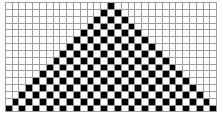
\includegraphics[]{img/wolframResult-15}
\caption{Result automata}
\end{figure}

This gives the result in figure 2. In this case the result is very well structured and organized. Wolfram discovered that there are 256 of these simple sets of rules, based on eight individual rules. Not every one of these 256 sets gives nicely structured results.

\paragraph{Music}

Wolfram used his automata to create music. Let's say we used one of the 256 sets of rules to create a result pattern. We can take a partition through this pattern of 15 cells wide. When we flip this partition on its side we can treat it as a musical score.
Figure 3 shows the partition from a resulting pattern and figure 4 shows it as a musical score.

 \begin{figure}[h]
\centering
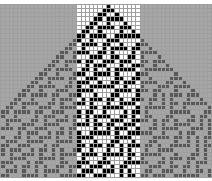
\includegraphics[]{img/wolframMusic1}
\caption{Partition through pattern}
\end{figure}

\begin{figure}[h]
\centering
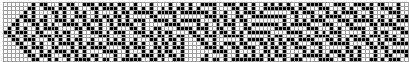
\includegraphics[]{img/wolframMusic2}
\caption{Musical score}
\end{figure}

Now we can assume that time runs across the page from left to right and every black cell represents a note played. Wolfram has developed his own programming language and uses various of his own algorithms to form music out of these cellular automaton patterns.
\newline
\newline
The number of rules isn't limited by eight individual rules. We can determine the color of the next cell by looking at his five upper row neighbours, instead of three. This gives a much bigger number of results (around 4 billion) and much more interesting results to use in the music creation. 

\subsubsection{Genetic algorithms}

Another interesting case to focus on is the use of genetic algorithms to produce music, as explained in the paper by Dragan Matic [2].
\newline

A genetic algorithm is an algorithm based on the idea of natural selection. The execution of a genetic algorithm starts with an initial population of individuals. During the execution of the algorithm, it will try and find an optimal solution based on predetermined rules. Each indiviual of the population has an attribute 'fitness'. This attribute denotes the quality of each individual of the population.
\newline

This particular GA used in the paper of Dragan Matic uses complete compositions as the individuals of the population. A composition is any combination of rhythm and notes, the concept of good and bad music is represented in the fitness attribute. Because the notion of good and bad music is very subjective and different for each person, Matic uses a reference individual for the evaluation of the resulting composition.
\newline

We start with the initial population, containing $n$ individuals. After this, an iterative process begins. The fitness of each individual is calculated in each iteration. Based on the best individual (best fitness), we test if the stop condition is met. This stop condition can be set by the user before execution. If the algorithm decides to stop, the best individual is played.

If the algorithm continues, we remove two-thirds of the individuals in the population. Mutation operators are applied to the remaining individuals to generate new different individuals. Now the next iteration starts and we calculate the fitness of the new individuals and test if we have found a good composition.

\subsubsection{Computoser}

Computoser is a web application that generates random music. It is based on a rule-based, probability-driven algorithm. This means that it composes by following a set of rules and decisions between several alternatives that are based on predefined probabilities.
\newline

Computoser gives probabilities to every type of interval in music theory and to each note length.
An interval in music is the distance between two consecutive played notes, e.g. a fifth is a distance of five notes in the scale and gets a probability of 25\%. This is fairly high because it is very commonly used in composing.
\newline

Computoser uses seven groups of rules.
\begin{enumerate}
\item Structure
\item Rhythm
\item Repetition
\item Variations
\item Dissonance and syncopation
\item Endings
\item Effects
\end{enumerate}

Analogous to the probabilities given to intervals, each of the rules used in the algorithm has a certain percentage that decides which rule to use.
\newline

The components of the Computoser algorithm are called manipulators. They each fill in a part of information of the score. Analogous to the Unit Generators of the Beads library, these work as a chain. Subsequent manipulators depend on previous ones. There are four main manipulators.

\begin{enumerate}
\item Part configurer: what parts are there in the piece? Is there a bass line, a piano part?
\item Scale configurer: what scale is the piece in? The most likely scales are the major and minor scales. Scales like the Dorian are less likely.
\item Meter configurer: what meter is the piece in? 4/4 is the most common meter, but you can have a piece in 6/8, 3/4, etc.
\item Each part has its own generator and decides for each part what notes to play.
\end{enumerate}
 
The part generator is obviously the most important part of the algorithm, because it decides what notes to play. There are three main aspects to the generator. The decisions are all based on the idea of probability.

\paragraph{Pitch} Apart form using the probabilities there are a few other constraints used to determine what note to play next. First, there should not be more than two subsequent unstable notes. Secondly, long jumps (more than 7 steps) require a step in the opposition direction. Thirdly, a predefined sequence of notes may be used, if they are from the circle of fifths or part of an extended chord.

\paragraph{Length} Here are the probabilities used as well, but again some other constraints are used. First is the measure size, all measures should have the same length. The second constraint is rhythm. Each measure is either simple (only one down-beat, e.g. 2/4) or compound (more than one down-beat, e.g. 4/4).

\paragraph{Variation} Computoser uses motifs to construct the parts. There are a few simple motifs that we use as a basis. These motifs can undergo several musical variations to create new motifs. A few of these are transposition, all notes go higher or lower within the same scale. You have inversion, turning the melody 'upside-down', you have retrograding, playing the motif backwards, etc.
\newline

This is a quick rundown of how the Computoser algorithm works. There is more going on in the algorithm but that is out of scope of this paper.
 
\subsection{Chords and progressions}

A crucial element of music is the use of chord progressions. The most common example of this is a twelve bar blues. This type of music is characterised by a strict pattern. Every song that uses a twelve bar blues follows the same chord progression.

\begin{figure}[h]
\centering
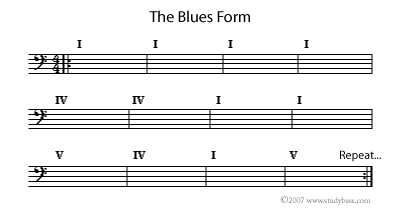
\includegraphics[]{img/the-blues-form}
\caption{Twelve bar blues}
\end{figure}

In figure 5 you can see the structure of a twelve bar blues, very simple yet very recognisable. The roman numbers denote which chord will be played, relatively to the key of the song.

There are many other kinds of progressions, such as the I-II-V-I chord progression, or any other combination. Most popular songs use multiple chord progressions, one for the verse, one for the chorus and so on. 
\newline

In ArtToMusic I will be using some standard chord progressions and some more unusual ones. There are a few reasons I choose for the use of chord progressions. Firstly, it is the most common way to write music. Secondly, it facilitates the generation of music in code. Several progressions are known to the ArtToMusic program and can be played easily, given the key of the song. 
‌\newline

A few of these standard chord progressions are the following:
\begin{itemize}
\item I-II-V-I: happy, vibrant
\item I-V-VI-IV: neutral
\item I-IV-I-V: very happy, upbeat
\end{itemize} 

To make matters more interesting, I can use some famous numbers from mathematics, such as $\pi$, $\phi$ and $e$. These irrational numbers can be seen as a series of digits. These digits can be seen as chords in a progression. For example, the first five digits of $\pi$ are 3, 1, 4, 5, and 1. When we see them as chords we get the following chord progression: III-I-IV-V-I, which seems a very interesting progression.
\newline

Analogous to the example we can use the digits of the other numbers and create many progressions based on the graphical analysis.

\section{Conclusion}

\begin{thebibliography}{1}

\bibitem{beads} Ollie Bown (http://www.beadsproject.net/) 2008

\bibitem{beads_sonifying} Evan X. Merz {\em Sonifying Processing: The Beads Tutorial} 2011

\bibitem{wolfram} Stephen Wolfram {\em A new kind of science} 2002

\bibitem{genetic} Dragan Mati\'c {\em A genetic algorithm for composing music} 2010, Faculty of Natural Sciences, University of Banjaluka, Bosnia and Herzegovina

\bibitem{computoser} Bozhidar Bozhanov {\em Computoser - rule-based, probability-driven algorithmic music composition} 2014,  independent researcher

\end{thebibliography}

\end{document}